
\chapter{Audio file formats and steganography techniques}

\begin{multicols}{2}
\section{Introduction}
Sound is the result of a vibration created by a phenomenon that propagates through a transmission environment, ending up getting interpreted by our brain. However since this process happens in the physical world it is entirely analog so it would be impossible to store it on modern day devices which can only understand digital formats. Luckily the fast evolution of computers also brought conversion techniques in order to switch between analog sounds and digital sounds seamlessly, without any noticeable loss to the human ear. Using these methods we have gained the ability to store audio files in a digital format so it was only logical that several different file formats will be created to fit our needs. In this chapter we will discuss in greater detail about how the analog data is actually stored in the digital format and what are the most common extensions used for storing digital audio files.

We mentioned earlier that it is impossible to store analog signals in a digital environment. The solution to this problem is to convert the audio signal which can be represented as a continuous-time function into a discrete-time function using a process called sampling. 

\begin{figure}[H]
    \centering
    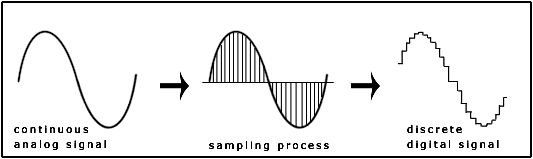
\includegraphics[width=7.7cm,keepaspectratio]{pics/Sampling-of-audio-signal.png}
    \caption{Converting a continuous signal into a discrete one\cite{real_time_audio_steganography}.}
    \label{sampling-graphic-example}
\end{figure}

The sampling process can be observed in figure \ref{sampling-graphic-example}. We can now introduce some new terms that we will use throughout the rest of the chapter:
\begin{itemize}
	\item \textbf{Sampling rate} is the number of samples taken per second, or in other terms, how many discrete values we store for each second of the audio signal. The measurement unit for sampling rate is Hertz (Hz for short) and some of the most common values are 44100, 48000 and some of their multiples.
	\item \textbf{Bit depth} is the number of bits used to store a single sample after having it converted to a discrete value. The most common bit depths are 8, 16, and 24 which allow for 256, 65536, and 16777216 different values. 
	\item \textbf{Audio channel} is the term used to describe the sequence of bytes that represent sampled audio signals. An audio file can have multiple channels to better simulate the sound accuracy and origin in a limited environment. Files with one audio channel are called mono, with two they become stereo and any more channels makes them surround. However, no matter the number of channels, usually all of them are equal in length and the samples from each channel are played simultaneously.
\end{itemize}

In the steganography field, the most common configuration that accepts alterations to the sampled data without losing any noticeable quality is a sampling rate of 44.1kHz with a bit depth of 16 and any number of audio channels, so this the ideal format that we will use throughout the rest of the chapter. The reason why this configuration is favored so much is because of the popularity that came with the invention of CDs and MP3s which used it as a default. Furthermore, any changes made to the sampled data are usually small enough that they will not be noticeable according to the Nyquist-Shannon sampling theorem \cite{Shannon1949}, which is used to compute the condition such that the conversion from a continuous signal to a discrete one will capture all the relevant information. Using the aforementioned theorem and armed with the knowledge that the human physiology enables us to hear audio signals ranging from 20Hz to 20kHz, we can see why the 44.1kHz sampling rate is ideal in audio steganography.
\section{Additional techniques used in audio steganography}
\subsection{Embedding within certain frequencies}
TO DO: talk about the frequency modulation inside audio files after having explained the digital audio format, the sampling rate, the sample depth. Westfeld et al. with Steganography for Radio Amateurs - A DSSS Based Approach for Slow Scan Television. Example of tools like audacity using Nyquist plugins for frequency modulation. 

\section{The MPEG-1/2 Audio Layer III (MP3)}
TO DO: research the MP3 format, how they store the audio samples, headers, compression, why it became so popular etc.

\section{Waveform Audio (WAV)}
The Waveform Audio format commonly known as WAV is a popular file format for storing high quality digital audio files originally built by Microsoft. It bears many similarities to the PNG format in the internal structure/composition of the file: both begin with a very specific sequence of bytes (also known as the magic bytes) that help classification applications identify them, are separated into multiple parts (also known as chunks) that have their purpose and are extremely common in the modern day multimedia.

TO DO: talk about the structure of the WAV format and the support for the steganography algorithms aforementioned.
\end{multicols}